\documentclass[11pt,a4paper]{article}

% Packages
\usepackage[utf8]{inputenc}
\usepackage[T1]{fontenc}
\usepackage{lmodern}
\usepackage[margin=1in]{geometry}
\usepackage{graphicx}
\usepackage{hyperref}
\usepackage{xcolor}
\usepackage{listings}
\usepackage{booktabs}
\usepackage{float}
\usepackage{enumitem}
\usepackage{amsmath}
\usepackage{tikz}
\usetikzlibrary{shapes.geometric, arrows.meta, positioning, fit, backgrounds}

% Colors
\definecolor{codegreen}{rgb}{0,0.6,0}
\definecolor{codegray}{rgb}{0.5,0.5,0.5}
\definecolor{codepurple}{rgb}{0.58,0,0.82}
\definecolor{backcolour}{rgb}{0.95,0.95,0.92}
\definecolor{attackblue}{RGB}{74,144,164}
\definecolor{neuralgreen}{RGB}{40,167,69}
\definecolor{symbolicorange}{RGB}{255,193,7}

% Code listing style
\lstdefinestyle{mystyle}{
    backgroundcolor=\color{backcolour},
    commentstyle=\color{codegreen},
    keywordstyle=\color{magenta},
    numberstyle=\tiny\color{codegray},
    stringstyle=\color{codepurple},
    basicstyle=\ttfamily\footnotesize,
    breakatwhitespace=false,
    breaklines=true,
    captionpos=b,
    keepspaces=true,
    numbers=left,
    numbersep=5pt,
    showspaces=false,
    showstringspaces=false,
    showtabs=false,
    tabsize=2,
    frame=single
}
\lstset{style=mystyle}

% Hyperref setup
\hypersetup{
    colorlinks=true,
    linkcolor=attackblue,
    filecolor=magenta,
    urlcolor=cyan,
    pdftitle={ATT\&CK Knowledge Graph Architecture},
    pdfauthor={},
}

% Title
\title{
    \textbf{ATT\&CK Knowledge Graph} \\
    \large A Neuro-Symbolic System for Threat Intelligence
}
\author{}
\date{\today}

\begin{document}

\maketitle

\begin{abstract}
The ATT\&CK Knowledge Graph is a neuro-symbolic system that combines MITRE ATT\&CK threat intelligence data as an RDF knowledge graph with vector embeddings for intelligent threat intelligence querying. This document describes the system architecture, data flow, and key design decisions that enable security teams to analyze attack narratives, identify relevant techniques, and receive remediation recommendations through both structured (SPARQL) and semantic (vector similarity) query mechanisms.
\end{abstract}

\tableofcontents
\newpage

%==============================================================================
\section{Introduction}
%==============================================================================

The MITRE ATT\&CK framework is an industry-standard knowledge base of adversary tactics, techniques, and procedures (TTPs). While the raw data is available in STIX 2.1 format, effectively querying and analyzing this information requires specialized tooling.

The ATT\&CK Knowledge Graph addresses this need by providing:
\begin{itemize}[noitemsep]
    \item Natural language querying of attack techniques
    \item Structured SPARQL queries over an RDF knowledge graph
    \item Hybrid neuro-symbolic queries combining both approaches
    \item LLM-powered analysis of security findings
    \item Automated remediation recommendations
\end{itemize}

\subsection{Design Philosophy}

The system follows a \textbf{neuro-symbolic} architecture, combining:
\begin{description}
    \item[Neural Component] Vector embeddings enable semantic similarity search, allowing queries like ``credential theft from memory'' to find relevant techniques without exact keyword matching.
    \item[Symbolic Component] An RDF knowledge graph provides structured relationships between entities (techniques, groups, software, mitigations), enabling precise graph traversals and SPARQL queries.
\end{description}

This dual approach leverages the strengths of both paradigms: neural networks excel at fuzzy matching and semantic understanding, while symbolic systems excel at precise reasoning over structured relationships.

%==============================================================================
\section{System Architecture}
%==============================================================================

Figure~\ref{fig:architecture} shows the high-level architecture of the system.

\begin{figure}[H]
\centering
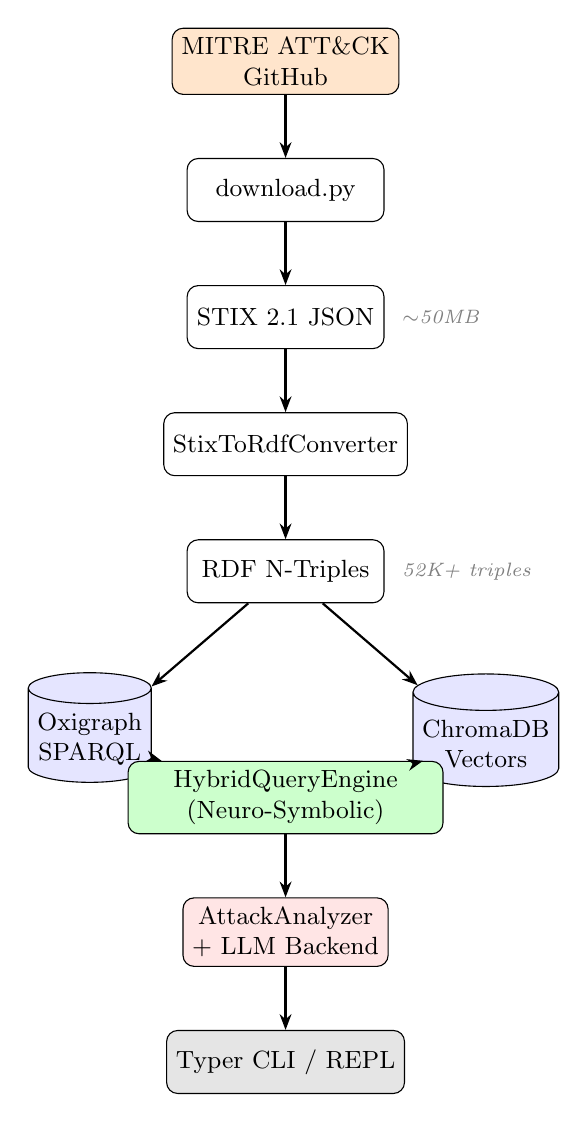
\begin{tikzpicture}[
    node distance=0.8cm,
    box/.style={rectangle, draw, rounded corners, minimum width=2.5cm, minimum height=0.8cm, align=center, font=\small},
    storage/.style={cylinder, draw, shape border rotate=90, aspect=0.25, minimum height=1.2cm, minimum width=1.5cm, align=center, font=\small},
    arrow/.style={-{Stealth[length=2mm]}, thick},
    label/.style={font=\scriptsize\itshape, text=gray}
]

% External
\node[box, fill=orange!20] (mitre) {MITRE ATT\&CK\\GitHub};

% Ingestion
\node[box, below=of mitre] (download) {download.py};
\node[box, below=of download] (stix) {STIX 2.1 JSON};
\node[box, below=of stix] (converter) {StixToRdfConverter};
\node[box, below=of converter] (rdf) {RDF N-Triples};

% Storage (side by side)
\node[storage, below left=1cm and 0.5cm of rdf, fill=blue!10] (oxigraph) {Oxigraph\\SPARQL};
\node[storage, below right=1cm and 0.5cm of rdf, fill=blue!10] (chroma) {ChromaDB\\Vectors};

% Query layer
\node[box, below=2cm of rdf, fill=green!20, minimum width=4cm] (hybrid) {HybridQueryEngine\\(Neuro-Symbolic)};

% Reasoning
\node[box, below=of hybrid, fill=red!10] (analyzer) {AttackAnalyzer\\+ LLM Backend};

% CLI
\node[box, below=of analyzer, fill=gray!20] (cli) {Typer CLI / REPL};

% Arrows
\draw[arrow] (mitre) -- (download);
\draw[arrow] (download) -- (stix);
\draw[arrow] (stix) -- (converter);
\draw[arrow] (converter) -- (rdf);
\draw[arrow] (rdf) -- (oxigraph);
\draw[arrow] (rdf) -- (chroma);
\draw[arrow] (oxigraph) -- (hybrid);
\draw[arrow] (chroma) -- (hybrid);
\draw[arrow] (hybrid) -- (analyzer);
\draw[arrow] (analyzer) -- (cli);

% Labels
\node[label, right=0.1cm of stix] {$\sim$50MB};
\node[label, right=0.1cm of rdf] {52K+ triples};

\end{tikzpicture}
\caption{High-level system architecture showing data flow from MITRE ATT\&CK through the ingestion pipeline to the query and reasoning layers.}
\label{fig:architecture}
\end{figure}

%==============================================================================
\section{Technology Stack}
%==============================================================================

\begin{table}[H]
\centering
\begin{tabular}{@{}lll@{}}
\toprule
\textbf{Layer} & \textbf{Technology} & \textbf{Purpose} \\
\midrule
Language & Python 3.11+ & Core implementation \\
CLI Framework & Typer & Command-line interface with rich formatting \\
RDF Store & Oxigraph (pyoxigraph) & SPARQL query engine \\
Vector Store & ChromaDB & Cosine similarity search \\
Embeddings & sentence-transformers & nomic-embed-text-v1.5 (8K context) \\
LLM (Local) & Ollama & Local model inference \\
LLM (Cloud) & OpenAI & GPT-4 API access \\
Data Format & STIX 2.1 $\rightarrow$ RDF & Threat intelligence representation \\
Package Manager & UV & Fast Python dependency management \\
Containerization & Docker & Multi-stage build for deployment \\
\bottomrule
\end{tabular}
\caption{Technology stack overview.}
\label{tab:techstack}
\end{table}

%==============================================================================
\section{Module Architecture}
%==============================================================================

The codebase is organized into four primary modules, each with distinct responsibilities.

\subsection{Ingest Module (\texttt{src/ingest/})}

Responsible for converting MITRE STIX data to an RDF knowledge graph.

\begin{description}
    \item[\texttt{download.py}] Downloads the STIX bundle from MITRE GitHub with progress indication.
    \item[\texttt{stix\_to\_rdf.py}] Two-pass converter that first processes entities (techniques, groups, software, mitigations, campaigns, tactics, data sources, data components, detection strategies, analytics) to build a STIX ID $\rightarrow$ URI mapping, then processes relationships using that mapping.
    \item[\texttt{embeddings.py}] Generates vector embeddings for technique descriptions using sentence-transformers and stores them in ChromaDB.
\end{description}

\subsubsection{Two-Pass Conversion Strategy}

The STIX-to-RDF conversion uses a two-pass approach:

\begin{enumerate}
    \item \textbf{Pass 1: Entity Processing} --- Parse all STIX objects (techniques, groups, software, mitigations, campaigns, tactics, data sources, data components, detection strategies, analytics) and create RDF entities. Build a mapping from STIX IDs to RDF URIs.
    \item \textbf{Pass 2: Relationship Processing} --- Process relationship objects (uses, mitigates, subtechniqueOf, detects, attributedTo, targets), using the ID mapping to resolve source and target references to valid URIs.
\end{enumerate}

This ensures that all entity URIs exist before creating relationships, avoiding dangling references.

\subsection{Store Module (\texttt{src/store/})}

Provides persistent storage abstractions for both structured and vector data.

\begin{description}
    \item[\texttt{graph.py}] \texttt{AttackGraph} class wrapping Oxigraph with 32 query methods. Provides:
    \begin{itemize}[noitemsep]
        \item RDF file loading (N-Triples, Turtle)
        \item SPARQL query execution
        \item Technique queries: \texttt{get\_technique()}, \texttt{get\_subtechniques()}, \texttt{get\_techniques\_for\_tactic()}
        \item Group queries: \texttt{get\_techniques\_for\_group()}, \texttt{get\_groups\_using\_technique()}
        \item Defense queries: \texttt{get\_mitigations\_for\_technique()}, \texttt{get\_detections\_for\_technique()}
        \item Campaign queries: \texttt{get\_campaign()}, \texttt{get\_techniques\_for\_campaign()}
        \item Data source queries: \texttt{get\_data\_sources()}, \texttt{get\_techniques\_by\_data\_source()}
    \end{itemize}

    \item[\texttt{vectors.py}] \texttt{SemanticSearch} class wrapping ChromaDB. Provides:
    \begin{itemize}[noitemsep]
        \item Vector similarity search
        \item Metadata filtering (tactic, platform)
        \item Returns \texttt{SemanticResult} objects with similarity scores
    \end{itemize}
\end{description}

\subsection{Query Module (\texttt{src/query/})}

Implements the neuro-symbolic query engine.

\begin{description}
    \item[\texttt{semantic.py}] \texttt{SemanticSearchEngine} for pure vector-based queries.
    \item[\texttt{sparql.py}] \texttt{QueryTemplates} with 20+ SPARQL patterns for common ATT\&CK queries.
    \item[\texttt{hybrid.py}] \texttt{HybridQueryEngine} --- the neuro-symbolic core combining vector search with SPARQL enrichment.
\end{description}

\subsubsection{HybridQueryEngine Capabilities}

The \texttt{HybridQueryEngine} is the central component providing five capability areas:

\begin{description}
    \item[Core Queries] Basic neuro-symbolic search: \texttt{query()}, \texttt{find\_defenses()}, \texttt{get\_threat\_context()}
    \item[Campaign Analysis] Threat campaign intelligence: \texttt{get\_campaign\_context()}, \texttt{find\_similar\_campaigns()}
    \item[Detection Analysis] Detection coverage mapping: \texttt{get\_detection\_coverage()}, \texttt{find\_by\_data\_source()}
    \item[Kill Chain Analysis] Attack progression analysis: \texttt{analyze\_kill\_chain()}, \texttt{get\_attack\_surface()}
    \item[Entity Search] Generic entity operations: \texttt{search\_entities()}, \texttt{get\_entity()}, \texttt{get\_relationships()}
\end{description}

\subsubsection{Hybrid Query Flow}

The neuro-symbolic pattern combines neural and symbolic approaches:

\begin{enumerate}
    \item \textbf{Vector Search:} Embed the query and find semantically similar techniques.
    \item \textbf{SPARQL Enrichment:} For each candidate, query the RDF graph for:
    \begin{itemize}[noitemsep]
        \item Associated tactics (kill chain phases)
        \item Threat groups and campaigns using the technique
        \item Available mitigations and detections
        \item Software implementations
        \item Parent/child technique relationships
        \item Data sources for detection
    \end{itemize}
    \item \textbf{Return Enriched Results:} \texttt{EnrichedTechnique} objects containing both semantic match data and structured graph context.
\end{enumerate}

\subsection{Reasoning Module (\texttt{src/reasoning/})}

LLM-powered analysis and remediation generation.

\begin{description}
    \item[\texttt{llm.py}] Abstract \texttt{LLMBackend} with implementations for Ollama (local) and OpenAI (cloud).
    \item[\texttt{analyzer.py}] \texttt{AttackAnalyzer} that:
    \begin{itemize}[noitemsep]
        \item Classifies security findings against candidate techniques
        \item Assigns confidence levels (high/medium/low)
        \item Extracts evidence from narratives
        \item Generates prioritized remediation recommendations
        \item Generates LLM-based detection recommendations using graph-stored data sources, detection strategies, and analytics as context
    \end{itemize}
\end{description}

%==============================================================================
\section{Knowledge Graph Schema}
%==============================================================================

\subsection{RDF Namespaces}

\begin{lstlisting}[language=,caption={RDF namespace prefixes}]
PREFIX attack: <https://attack.mitre.org/>
PREFIX rdfs:   <http://www.w3.org/2000/01/rdf-schema#>
PREFIX rdf:    <http://www.w3.org/1999/02/22-rdf-syntax-ns#>
\end{lstlisting}

\subsection{Entity Types}

\begin{table}[H]
\centering
\begin{tabular}{@{}lll@{}}
\toprule
\textbf{RDF Type} & \textbf{STIX Type} & \textbf{Description} \\
\midrule
\texttt{attack:Technique} & attack-pattern & Attack technique \\
\texttt{attack:Group} & intrusion-set & Threat actor group \\
\texttt{attack:Malware} & malware & Malicious software \\
\texttt{attack:Tool} & tool & Legitimate tool used maliciously \\
\texttt{attack:Mitigation} & course-of-action & Defensive measure \\
\texttt{attack:Tactic} & x-mitre-tactic & Kill chain phase \\
\texttt{attack:Campaign} & campaign & Threat campaign \\
\texttt{attack:DataSource} & x-mitre-data-source & Detection data source \\
\texttt{attack:DataComponent} & x-mitre-data-component & Detection data component \\
\texttt{attack:DetectionStrategy} & x-mitre-detection-strategy & Detection approach \\
\texttt{attack:Analytic} & x-mitre-analytic & Specific detection rule \\
\bottomrule
\end{tabular}
\caption{Mapping between RDF types and STIX types.}
\end{table}

\subsection{Key Properties}

\begin{table}[H]
\centering
\begin{tabular}{@{}ll@{}}
\toprule
\textbf{Property} & \textbf{Description} \\
\midrule
\texttt{attack:attackId} & ATT\&CK identifier (e.g., T1110.003) \\
\texttt{rdfs:label} & Human-readable name \\
\texttt{attack:description} & Full technique description \\
\texttt{attack:uses} / \texttt{attack:usedBy} & Group/software/campaign uses technique (+ inverse) \\
\texttt{attack:mitigates} / \texttt{attack:mitigatedBy} & Mitigation addresses technique (+ inverse) \\
\texttt{attack:subtechniqueOf} & Parent technique relationship \\
\texttt{attack:tactic} & Kill chain phase association \\
\texttt{attack:platform} & Target platform (Windows, Linux, etc.) \\
\texttt{attack:detects} / \texttt{attack:detectedBy} & Data component detects technique (+ inverse) \\
\texttt{attack:attributedTo} / \texttt{attack:hasCampaign} & Campaign attributed to group (+ inverse) \\
\texttt{attack:targets} & Technique targets asset \\
\texttt{attack:hasAnalytic} & Detection strategy has analytic \\
\bottomrule
\end{tabular}
\caption{Key RDF properties in the knowledge graph.}
\end{table}

\subsection{Example SPARQL Query}

\begin{lstlisting}[language=SQL,caption={SPARQL query to find technique details with mitigations}]
PREFIX attack: <https://attack.mitre.org/>
PREFIX rdfs: <http://www.w3.org/2000/01/rdf-schema#>

SELECT ?name ?tactic ?mitigation ?mitigationName WHERE {
  <https://attack.mitre.org/technique/T1110.003>
    rdfs:label ?name ;
    attack:tactic ?tactic .

  OPTIONAL {
    ?mitigation attack:mitigates
      <https://attack.mitre.org/technique/T1110.003> ;
      rdfs:label ?mitigationName .
  }
}
\end{lstlisting}

%==============================================================================
\section{Data Flow}
%==============================================================================

\subsection{Ingestion Pipeline}

\begin{enumerate}
    \item \textbf{Download:} Fetch \texttt{enterprise-attack.json} from MITRE GitHub ($\sim$50MB STIX bundle).
    \item \textbf{Parse:} Load JSON and extract STIX objects.
    \item \textbf{Convert (Pass 1):} Process entities, build ID$\rightarrow$URI mapping.
    \item \textbf{Convert (Pass 2):} Process relationships using the mapping.
    \item \textbf{Serialize:} Write RDF as N-Triples for fast loading.
    \item \textbf{Load Graph:} Bulk load into Oxigraph.
    \item \textbf{Generate Embeddings:} Extract techniques via SPARQL, embed descriptions, store in ChromaDB.
\end{enumerate}

\subsection{Query Pipeline}

Given a natural language query (e.g., ``Found password spraying attack''):

\begin{enumerate}
    \item \textbf{Embed Query:} Generate vector embedding using sentence-transformers.
    \item \textbf{Vector Search:} Find top-$k$ similar techniques in ChromaDB.
    \item \textbf{Graph Enrichment:} For each candidate, execute SPARQL queries to fetch:
    \begin{itemize}[noitemsep]
        \item Tactic associations
        \item Threat groups and campaigns using the technique
        \item Available mitigations
        \item Related software
        \item Sub-technique relationships
        \item Data sources and detection analytics
    \end{itemize}
    \item \textbf{LLM Classification:} Present enriched candidates to LLM for:
    \begin{itemize}[noitemsep]
        \item Confidence scoring
        \item Evidence extraction
        \item Technique selection
    \end{itemize}
    \item \textbf{Remediation \& Detection:} Generate prioritized mitigation and detection recommendations.
\end{enumerate}

%==============================================================================
\section{Knowledge Base Statistics}
%==============================================================================

After a full build, the knowledge graph contains:

\begin{table}[H]
\centering
\begin{tabular}{@{}lr@{}}
\toprule
\textbf{Entity Type} & \textbf{Count} \\
\midrule
Techniques (with sub-techniques) & $\sim$835 \\
Threat Groups & $\sim$187 \\
Software (malware + tools) & $\sim$787 \\
Mitigations & $\sim$268 \\
Campaigns & $\sim$52 \\
Tactics & 14 \\
Data Sources & $\sim$38 \\
Data Components & $\sim$109 \\
Detection Strategies & $\sim$691 \\
Analytics & $\sim$1,739 \\
RDF Triples (total) & varies \\
\bottomrule
\end{tabular}
\caption{Knowledge base statistics (approximate, varies by ATT\&CK version).}
\end{table}

%==============================================================================
\section{CLI Interface}
%==============================================================================

The system provides a Typer-based CLI with the following commands:

\begin{table}[H]
\centering
\begin{tabular}{@{}ll@{}}
\toprule
\textbf{Command} & \textbf{Description} \\
\midrule
\texttt{download} & Fetch STIX bundle from MITRE \\
\texttt{ingest} & Convert STIX to RDF \\
\texttt{build} & Load RDF and build vector index \\
\texttt{stats} & Display knowledge graph statistics \\
\texttt{query} & Execute raw SPARQL queries \\
\texttt{technique} & Get technique details by ID \\
\texttt{group} & Get group's techniques \\
\texttt{search} & Semantic search for techniques \\
\texttt{analyze} & Analyze narrative and suggest remediations \\
\texttt{repl} & Interactive session with history \\
\bottomrule
\end{tabular}
\caption{CLI commands.}
\end{table}

\subsection{Usage Examples}

\begin{lstlisting}[language=bash,caption={CLI usage examples}]
# Data pipeline
uv run attack-kg download
uv run attack-kg ingest
uv run attack-kg build

# Lookups
uv run attack-kg technique T1110.003
uv run attack-kg group APT29

# Semantic search
uv run attack-kg search "credential theft from memory"

# Full analysis
uv run attack-kg analyze "Found password spraying attack"
uv run attack-kg analyze --file finding.txt --backend openai
\end{lstlisting}

%==============================================================================
\section{Design Decisions}
%==============================================================================

\begin{table}[H]
\centering
\begin{tabular}{@{}p{4cm}p{9cm}@{}}
\toprule
\textbf{Decision} & \textbf{Rationale} \\
\midrule
Oxigraph over oxrdflib & oxrdflib had hanging issues; pyoxigraph provides direct, performant SPARQL access \\
N-Triples over Turtle & 10--30$\times$ faster loading; sacrifices human readability for performance \\
Two-pass STIX conversion & Ensures all entity URIs exist before linking relationships \\
nomic-embed-text-v1.5 & 8K token context handles long technique descriptions \\
ChromaDB over cloud vectors & Local, persistent, no API keys required \\
Full URIs in SPARQL & ATT\&CK IDs with dots (T1110.003) break prefix notation \\
Lazy-load LLM backends & REPL can function without LLM initialization overhead \\
\bottomrule
\end{tabular}
\caption{Key design decisions and their rationale.}
\end{table}

%==============================================================================
\section{Deployment}
%==============================================================================

\subsection{Docker}

The system uses a multi-stage Docker build:

\begin{enumerate}
    \item \textbf{Builder Stage:} Downloads STIX data, builds knowledge graph, installs dependencies.
    \item \textbf{Runtime Stage:} Slim image with pre-built stores for fast startup.
\end{enumerate}

\subsection{Environment Variables}

\begin{table}[H]
\centering
\begin{tabular}{@{}ll@{}}
\toprule
\textbf{Variable} & \textbf{Description} \\
\midrule
\texttt{OLLAMA\_HOST} & Ollama server URL (default: \texttt{http://localhost:11434}) \\
\texttt{OPENAI\_API\_KEY} & OpenAI API key for cloud LLM \\
\bottomrule
\end{tabular}
\caption{Environment variables.}
\end{table}

%==============================================================================
\section{Conclusion}
%==============================================================================

The ATT\&CK Knowledge Graph demonstrates the power of neuro-symbolic architectures for threat intelligence. By combining vector similarity search with structured RDF graph queries, the system provides flexible, powerful querying capabilities that would be difficult to achieve with either approach alone.

The modular architecture separates concerns cleanly:
\begin{itemize}[noitemsep]
    \item \textbf{Ingest} handles data transformation
    \item \textbf{Store} manages persistence
    \item \textbf{Query} implements the hybrid search logic
    \item \textbf{Reasoning} adds LLM intelligence
\end{itemize}

This separation enables independent evolution of each component while maintaining a cohesive system for security analysts.

\end{document}
